\subsection{CoSimComponent Interface}
\label{sec:architecture_cosimcomponent}

The \texttt{CoSimComponent} interface defines the architectural contract for simulation components in \syssimx{}.
It separates backend-specific model behavior from framework-level orchestration.
All components expose the same interface for initialization, stepping, data exchange, and result collection.
This uniform contract follows from the co-simulation formulation in Section~\ref{sec:232_cosim_formulation}.

The master algorithms require a component interface with four properties.
Components must expose typed and unit-aware ports.
They must support a common lifecycle for initialization and stepping.
They must declare the input-output dependencies needed for structural analysis.
Components that participate in hybrid scenarios must also provide the state handling needed for rollback.
Figure~\ref{fig:cosimcomponent_architecture} summarizes this interface.

\begin{figure}[t]
  \centering
  \vspace{-1em}
  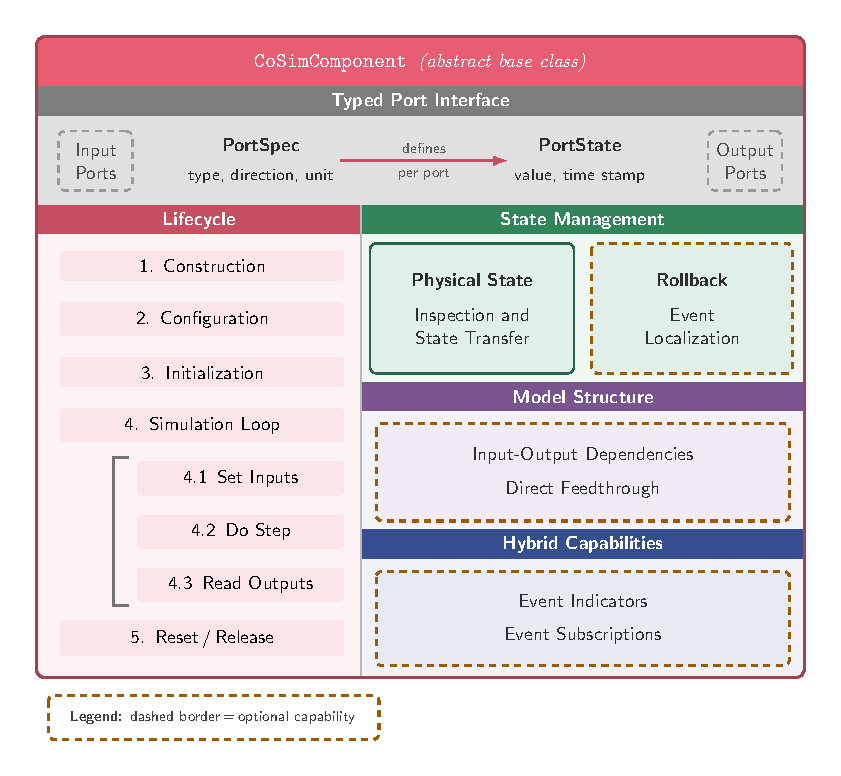
\includegraphics[width=0.95\textwidth]{figures/4_architecture/cosimcomponent.pdf}
  \vspace{-1em}
  \caption{Architectural overview of the \texttt{CoSimComponent} interface.
  The interface combines typed ports, a common lifecycle, state handling, and optional capabilities for structural analysis and hybrid co-simulation.}
  \vspace{-0.5em}
  \label{fig:cosimcomponent_architecture}
\end{figure}

\paragraph{Typed Port Interface.}
A component exposes its system interface through typed input and output ports.
Each port carries a declared data type and an optional physical unit.
These declarations make coupling assumptions explicit at the interface level.
They also allow the framework to validate type compatibility and unit consistency when connections are established, as described in Section~\ref{sec:architecture_system_connections}.

\paragraph{Lifecycle and Inversion of Control.}
The interface prescribes a common lifecycle for all components.
A component is constructed, configured, initialized at the simulation start time, stepped during the simulation loop, and reset or finalized after use.
The framework owns this lifecycle order.
Backend-specific subclasses provide the model operations that are called inside this order.

This inversion of control keeps framework concerns in one place.
Port-state management, time bookkeeping, history recording, and capability checks are handled uniformly.
Backend wrappers can focus on model-specific initialization, stepping, and output evaluation.

\paragraph{Declared Structural and Hybrid Metadata.}
The component interface also exposes metadata needed by the system-level orchestration.
The direct-feedthrough declaration states which outputs can depend on which inputs within the same communication step.
The \texttt{System} abstraction uses this information together with the connection structure to derive the execution constraints described in Section~\ref{sec:233_cosim_structural_analysis}.

Hybrid components can additionally expose event indicators and event subscriptions.
Event indicators allow an algorithm to detect and localize discrete events.
Event subscriptions define which components must receive an event after it has been detected.

\paragraph{State Handling.}
The interface separates physical state transfer from rollback state transfer.
Physical state transfer exports semantically meaningful quantities such as positions, velocities, or mode indicators.
It is used for inspection and for synchronization between alternative models of the same subsystem.

Rollback state transfer captures and restores the internal solver state of a component.
It is used during hybrid event handling, where the simulation may have to return to an earlier time and re-advance.
The two mechanisms are separated because rollback state is tool-specific, while physical state must remain meaningful across model representations.

\paragraph{Opt-in Capabilities.}
Components do not have to support every advanced capability.
The lifecycle operations are mandatory.
Physical state transfer, rollback, zero-step output evaluation, event indicators, and event handling are optional.
This keeps simple components lightweight and limits additional complexity to components that participate in strongly coupled or hybrid scenarios.